%\section{What is Bulk IO?}
\section{Bulk IO}
\label{sec:bulkio}

The typical mechanism for iterating through data in a \texttt{TTree} is a handwritten for-loop. ROOT uses a API shown in Listing \ref{getentry} to read objects from a branch (TTree is a structure that contains one or multiple TBranches). This function runs in two steps. First, it searches the underlying storage medium for the basket where the event is located and then read the basket into a memory buffer. The TBasket is the data structure that represents the in-memory buffer. ROOT decompresses the buffer and put the uncompressed buffer in so-called ``kernel" space. In the second step, once the basket appears in memory,  GetEntry deserializes the requested event from the kernel-space buffer and copy it to user-space buffer.

\vspace{5pt}
\lstset{language=C++,
                basicstyle=\ttfamily,
                keywordstyle=\color{blue}\ttfamily,
                stringstyle=\color{red}\ttfamily,
                commentstyle=\color{green}\ttfamily,
                morecomment=[l][\color{magenta}]{\#},
                xleftmargin=.2\textwidth, xrightmargin=.2\textwidth,
                frame=single
}
\begin{lstlisting}[caption={GetEntry in TBranch.},captionpos=b, label={getentry}]
TBranch::GetEntry(Long64_t entry)
\end{lstlisting}

When user application is computationally expensive, the cost of library calls, frequently deserializing objects and copying data between memory buffers are amortized to effectively noting. Accordingly, we introduce a new interface for ROOT to copy all events in an on-disk \texttt{TBasket} directly to a user-provided memory buffer. For the simplest of cases - primitives and C-style arrays of primitives - where the serialization can be done without a separate buffer or ``fixing up" pointer contents, the user can request the serialized data be delivered to the buffer or deserialized data.  By requesting the serialized data directly and deserializing directly in the event loop, the user can avoid an expensive scan from main memory.

Pragmatically, the user will not implement code for deserializing data themselves: rather, we have provided a header-only C++ facade around the data, allowing the user to work with a proxy object.  This allows the compiler to inline the deserialization code in the correct place.

%Bulk I/O is a set of techniques and APIs that was developed for ROOT to allow the user to deserialize a broad set of events at a time. Each basket, visualized in \cite{bulk} is compressed and written to the file.  The main goal is that bulk IO allows the user to read all the objects in a basket at once.

%\begin{figure}[h]
%\centering
%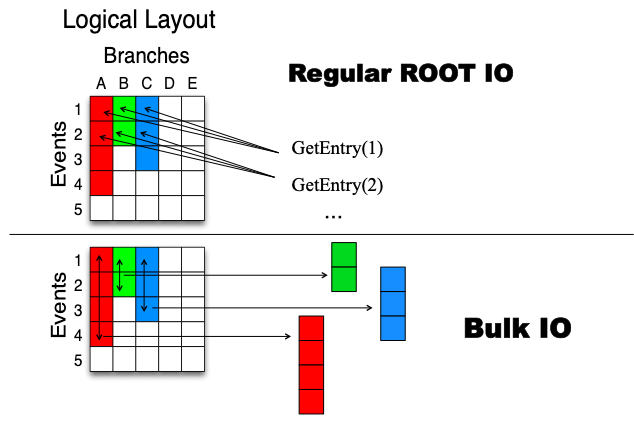
\includegraphics[width=0.7\linewidth]{bulk.png}
%\caption{ROOT I/O vs Bulk I/O schema.}
%\label{fig:bulk}
%\end{figure}

%Bulk IO can only work with a limited number of cases. It can only manipulate the data in-place, meaning the deserialized object in memory must be smaller than-or-equal-to the serialized byte stream. 

%Examples of  particular cases where bulk I/O can benefit the most:
%\begin{itemize}
%   \item Primitive types.
%   \item C-style structs and nothing with virtual pointers.
%   \item Arrays or std::vector of basic types.
%   \item No references or pointers.
%\end{itemize}

%\subsection{Pro \& cons for Bulk IO}

%For small and simple events, the overhead of ROOT library calls is much more significant than the cost of serialization itself. Bulk I/O is an approach to deliver a cluster of events at once. Further improvements can be achieved by returning serialized events to the user and allowing the compiler to inline deserialization in the event loop.

%Complex objects involving references or from polymorphic classes require expensive lookups to deserialize. In these cases, the library overheads are minimal, and bulk IO provides a little benefit.